% Paper draft: COVER (knowledge-grounded coverage/conflict NLI), formatted for ACL 2027
% (submitted through ACL Rolling Review; official *ACL style files from
% https://github.com/acl-org/acl-style-files: acl.sty, acl_natbib.bst).
% Build:  cd paper && latexmk -pdf main.tex      (clean: latexmk -C)
% Long paper: 8 pages of content (+1 in the camera-ready); Limitations, references and
% appendices do not count. "review" = anonymous, line numbers; "final" = camera-ready;
% "preprint" = non-anonymous with page numbers.
\documentclass[11pt]{article}
\usepackage[review]{acl}   % loads geometry, natbib, hyperref, caption, xcolor

% Standard packages of the ACL template
\usepackage{times}
\usepackage{latexsym}
\usepackage[T1]{fontenc}
\usepackage[utf8]{inputenc}
\usepackage{microtype}
\usepackage{inconsolata}
\usepackage{graphicx}

% Paper packages
\usepackage{amsmath,amssymb,bm}
\usepackage{tikz}
% TikZ figures in figures/*.tex are standalone documents; their preambles (colours, styles) are
% loaded automatically, so each figure can also be compiled on its own.
\usepackage[subpreambles=true]{standalone}
\usepackage{booktabs,multirow,array}
\usepackage{placeins}
\usepackage[capitalise,noabbrev]{cleveref}

% ---------------------------------------------------------------- notation
% Shared macros. Change \model once to rename the architecture everywhere.
\newcommand{\model}{COVER}
\newcommand{\todo}[1]{\textcolor{red}{[TODO: #1]}}

% Labels and sets
\newcommand{\E}{\textsc{e}}
\newcommand{\N}{\textsc{n}}
\newcommand{\C}{\textsc{c}}
\newcommand{\Prem}{\mathcal{P}}
\newcommand{\Hyp}{\mathcal{H}}
\newcommand{\Rel}{\mathcal{R}}
\newcommand{\Ops}{\mathcal{O}}
\newcommand{\cls}{\textsc{[cls]}}
\newcommand{\nullnode}{\varnothing}
\newcommand{\Lset}{\mathcal{L}_{\mathrm{set}}}
\newcommand{\Pcov}{P_{\mathrm{cov}}}
\newcommand{\Pnc}{P_{\neg\mathrm{conf}}}
\newcommand{\LN}{\operatorname{LN}}
\newcommand{\MLP}{\operatorname{MLP}}
\newcommand{\softplus}{\operatorname{softplus}}
\newcommand{\vect}[1]{\bm{#1}}
\providecommand{\best}[1]{\textbf{#1}}  % best value of a column in the result tables (boxed in the slides)


\title{\model: Knowledge-Grounded Coverage and Conflict Reasoning\\for Natural Language Inference in English and Portuguese}

% Hidden by the "review" option (anonymous submission).
\author{Antonio \textit{et al.} \\
  \todo{affiliation} \\
  \texttt{\todo{email}}}

\begin{document}
\maketitle

\begin{abstract}
\todo{Write last.}
\end{abstract}

\section{Introduction}
\label{sec:intro}

Natural language inference (NLI) asks whether a premise entails, contradicts or is neutral to a
hypothesis. Fine-tuned Transformer encoders reach high accuracy on standard benchmarks, but much of it
comes from annotation artifacts and shallow heuristics such as lexical overlap
\citep{gururangan2018annotation,mccoy2019right}; accuracy drops on diagnostic and challenge sets that
isolate a single phenomenon \citep{glockner2018breaking,wang2019superglue}.

The labels themselves have a simple logical reading. A hypothesis is entailed when \emph{every} part of
it is supported by the premise and \emph{no} part conflicts with it; one conflicting part makes it a
contradiction; otherwise it is neutral. A cross-encoder that classifies the pair from a single pooled
vector is free to ignore this structure, and nothing in its output shows which words drove the decision.

Two lines of work address these problems separately. Knowledge-enhanced models inject lexical or
knowledge-graph relations into the encoder \citep{chen2018neural,liu2020kbert,song2020kganet,wang2020knowledge},
but the evidence enters as an extra feature and does not change how the label is reached. Atomic-inference
models decide the label from per-span predictions and logical rules \citep{stacey2022logical,wu2023weakly},
but rely on span segmentation and use no external knowledge.

We propose \model{} (Knowledge-Grounded \emph{COVE}rage and Conflict \emph{R}easoning), which combines
both ideas on top of any pretrained encoder. Content words of the pair become nodes of a token graph whose
edges are typed lexical relations (synonymy, hypernymy, antonymy, numbers) from WordNet, PT-LKB,
Wiktionary and rules. Relation-aware attention lets each hypothesis word look for its counterpart in the
premise, or for none.

Each hypothesis word then receives a support, a conflict and an importance score. A weighted product of
supports (coverage) and a noisy-OR of conflicts define a structured distribution over the three labels,
which is added to the logits of the standard \cls{} classifier. The new modules add about 2M parameters,
and their per-word scores explain each decision (\cref{fig:interpretability}).

We evaluate \model{} in English and Portuguese with large encoders: RoBERTa-large trained on SICK,
Albertina-900M trained on InferBR, and XLM-R-large transferred across the two languages. Every system,
including three re-implemented knowledge-graph baselines, is trained with the same fixed hyperparameters
and 10 seeds, and compared with paired tests on in-distribution, out-of-distribution and challenge sets.

\model{} matches the \cls{} baseline in distribution and improves on it out of distribution: by 4.9 to
8.6 MCC points on AX-b, ConjNLI and FraCaS in English, and by 2.3 points on ASSIN~2 and SICK-BR in
Portuguese, with about half the standard deviation across seeds. In English it also outperforms the
three knowledge-graph baselines out of distribution. \todo{cross-lingual summary when experiment 0014 finishes.}

Our contributions are:
(i)~\model{}, an encoder-agnostic architecture that grounds a coverage--conflict decision rule in typed
lexical relations over contextual token states;
(ii)~a controlled evaluation in English, Portuguese and cross-lingual transfer, with 10 seeds, paired
tests and knowledge-graph baselines;
(iii)~an ablation showing that coverage, not conflict, produces the gains, and an AX-b analysis of the
phenomena where coverage helps and fails;
(iv)~word-level explanations read directly from the model.
\todo{code and data release.}

% ===================================================================== Related Work
\section{Related Work}
\label{sec:related}

\subsection{External knowledge in NLI}
\label{sec:rw-knowledge}

Lexical knowledge has long been used to decide whether a hypothesis word is licensed by the premise.
KIM~\citep{chen2018neural} feeds WordNet relations (synonymy, antonymy, hypernymy, hyponymy,
co-hyponymy) as pairwise features into the co-attention, local inference and composition steps of ESIM,
and \citet{glockner2018breaking} showed that models trained on SNLI fail on pairs that differ by a
single lexical substitution, precisely the cases where such knowledge should help.

With pretrained
Transformers, knowledge is usually injected either as text or as entity embeddings: K-BERT
\citep{liu2020kbert} appends knowledge-graph triples to the input and restricts their visibility in
self-attention, while KnowBert~\citep{peters2019knowledge} and ERNIE~\citep{zhang2019ernie} link
mentions to knowledge-base entity embeddings.

Graph-based approaches retrieve a subgraph for the pair
and encode it with a graph neural network whose output is fused with the sentence representation
\citep{kapanipathi2020infusing}. KGAnet~\citep{song2020kganet} encodes the retrieved knowledge graph with
graph attention, and KGNLI~\citep{wang2020knowledge} processes the sentence pair and its knowledge in
separate semantic and knowledge branches.

A common limitation is that the retrieved evidence is used as an additional feature vector: it does not
change \emph{how} the decision is reached, and its effect on strong pretrained encoders is often small.
In \model{}, typed relations bias the premise--hypothesis alignment and enter the messages that each
hypothesis word receives, and the resulting word-level evidence is combined by explicit logical rules.

\subsection{Structure inside pretrained encoders}
\label{sec:rw-structure}

A second line of work integrates graphs with pretrained language models more tightly.
QA-GNN~\citep{yasunaga2021qagnn} reasons jointly over a question--answer context node and a
knowledge-graph subgraph, GreaseLM~\citep{zhang2022greaselm} exchanges information between the
language model and a graph neural network at several layers, and structural adapters
\citep{ribeiro2021structadapt} insert graph convolutions between frozen Transformer blocks.

These methods
target question answering or generation over knowledge or semantic graphs. \model{} instead builds its
graph over the contextual states of the encoder itself, connecting premise and hypothesis words through
lexical relations, and keeps the encoder untouched: the graph operates as a separate expert whose output
is added to the classifier logits.

\subsection{Alignment and natural logic}
\label{sec:rw-alignment}

Alignment between premise and hypothesis is a classic ingredient of NLI, from phrase-based aligners
\citep{maccartney2008phrase} to the soft attention of the decomposable attention model
\citep{parikh2016decomposable} and ESIM~\citep{chen2017enhanced}, whose matching features
($[\vect{x};\vect{m};\vect{x}\odot\vect{m};|\vect{x}-\vect{m}|]$) we reuse in the update of
\cref{eq:update}.

Natural logic~\citep{maccartney2009extended} goes further and composes lexical
relations along an alignment, taking into account the monotonicity of the context; NaturalLI
\citep{angeli2014naturalli} uses it for large-scale inference, and recent work makes the composition
differentiable \citep{feng2020exploring} or trains it with reinforcement learning and lexical resources
\citep{feng2022neuro}.

These systems depend on external aligners or polarity parsers that are mostly
available for English. \model{} uses a learned soft alignment with a \emph{null} target and does not model
monotonicity explicitly; the weakness this causes on downward-monotone contexts is discussed in
\cref{sec:results}.

\subsection{Atomic and probabilistic inference}
\label{sec:rw-atomic}

The aggregation in \model{} is closest to models that decide NLI from the parts of the hypothesis.
\citet{glickman2005probabilistic} defined the probability that a text entails a hypothesis as the product,
over hypothesis words, of the probability that each word is entailed by some text word, an idea later
extended by \citet{shnarch2011probabilistic}.

In neural NLI, SLR-NLI~\citep{stacey2022logical} treats
hypothesis spans as logical atoms, predicts a label for each span from sentence-level supervision, and
derives the pair label with rules such as ``a contradiction requires at least one contradicting span'';
it retains in-distribution accuracy and improves robustness when training data is scarce.

EPR~\citep{wu2023weakly} aligns phrases of the two sentences, predicts a label per aligned pair and
induces the sentence label with differentiable fuzzy-logic formulas, and FGLR~\citep{stacey2024atomic}
applies the same principle to facts generated by a large language model.

\model{} shares the decision rule of these models (any conflict yields contradiction; full support
yields entailment) but differs in three respects. First, its atoms are contextual token nodes rather than
spans, phrases or generated facts, so no chunker or generator is needed. Second, the alignment and the
messages of these atoms are shaped by typed lexical relations.

Third, the structured distribution is fused with, rather than substituted for, the sentence-level
classifier, which keeps phenomena that the rules cannot express within reach of the encoder.
\todo{confirm in the SLR-NLI and EPR papers whether either combines its prediction with a sentence-level
classifier or uses external knowledge.}

\subsection{Robustness and diagnostic evaluation}
\label{sec:rw-robustness}

NLI models exploit annotation artifacts \citep{gururangan2018annotation} and shallow heuristics such as
lexical overlap \citep{mccoy2019right}, so in-distribution accuracy overstates their inferential ability.

Diagnostic sets address this by annotating pairs with the phenomenon they test: the GLUE/SuperGLUE
diagnostic~\citep{wang2018glue,wang2019superglue}, which we use as AX-b, covers lexical semantics,
predicate--argument structure, logic and world knowledge, and MED~\citep{yanaka2019can} shows that models
fine-tuned on standard data handle upward but not downward monotonicity. Following this line, we report
results on out-of-distribution and diagnostic test sets in addition to in-distribution accuracy, and
analyse AX-b by phenomenon.

\subsection{NLI for Portuguese}
\label{sec:rw-portuguese}

Portuguese NLI has been driven by shared tasks and translated resources: ASSIN \citep{fonseca2016assin}
annotates entailment and paraphrase in news, SICK-BR~\citep{real2018sickbr} translates SICK, and ASSIN~2
\citep{real2020assin2} builds on SICK-BR with a binary entailment label. InferBR \citep{inferbr2024} provides
three-way labels and is the main benchmark of this work.

Most recent systems fine-tune Portuguese or
multilingual encoders such as BERTimbau~\citep{souza2020bertimbau}, Albertina~\citep{rodrigues2023albertina}
and XLM-R~\citep{conneau2020unsupervised}, and cross-lingual evaluation typically relies on XNLI
\citep{conneau2018xnli}, which does not include Portuguese.

Lexical-semantic resources for Portuguese
are comparatively rich, from Onto.PT~\citep{goncalooliveira2014ontopt} to PT-LKB
\citep{goncalooliveira2018ptlkb}, which merges ten resources, but to our knowledge they have not been
integrated into the inference mechanism of Transformer-based NLI models. \todo{check this claim with a
targeted search before submission.} \model{} uses PT-LKB in this way, and we also test whether the effect
transfers between English and Portuguese.

% ===================================================================== Methodology
% Every equation below mirrors src/graphnli_axb/models_tokgraph.py (CoveragePartialLabelClassifier,
% BipartiteRelationalLayer) and src/graphnli_axb/token_graph.py (graph construction).
% If the code changes, update this section.
\section{Methodology}
\label{sec:method}

\subsection{Task formulation}
\label{sec:task}

Given a premise $\Prem$ and a hypothesis $\Hyp$, natural language inference (NLI) asks whether $\Prem$
entails $\Hyp$ (\E), contradicts it (\C), or neither (\N). Some corpora only distinguish entailment from
its absence; we keep a single three-way output space $\mathcal{Y}=\{\E,\N,\C\}$ and evaluate two-way
corpora through the induced binary decision \E{} \emph{vs.} $\neg$\E{} (\cref{sec:protocol}).

Our design starts from a simple observation about the label semantics. A hypothesis is entailed when
\emph{every} part of it is supported by the premise and \emph{no} part of it conflicts with the premise;
it is contradicted as soon as \emph{one} part conflicts; otherwise it is neutral.

This view goes back to
probabilistic lexical entailment~\citep{glickman2005probabilistic}, where $P(\Hyp\mid\Prem)$ is a
product over hypothesis words, and to recent atomic-inference models that predict a label per
hypothesis span and combine them with logical rules~\citep{stacey2022logical,wu2023weakly}.
\model{} implements it over \emph{contextual token states} and grounds the per-word decisions in
\emph{typed lexical knowledge}.

\subsection{The \model{} architecture}
\label{sec:architecture}

\begin{figure*}[t]
  \centering
  \includestandalone[width=\textwidth]{figures/cover_architecture}
  \caption{\model{}. (a)~Token graph with typed lexical relations $r_{ij}$. (b)~Pretrained encoder.
  (c)~Bipartite relational attention, with a \emph{null} target. (d)~Support $s_k$, conflict $c_k$ and
  importance $\omega_k$ per hypothesis node. (e)~Coverage and noisy-OR conflict give a distribution $z$,
  added to the \cls{} logits. \todo{update panel (a): operator scope edges are built but not used by \model.}}
  \label{fig:architecture}
\end{figure*}

\Cref{fig:architecture} gives an overview. \model{} keeps the standard cross-encoder classifier and
adds a structured expert whose output is a log-probability distribution over $\mathcal{Y}$. The expert
has three parts: a token graph built from symbolic resources (\cref{sec:graph}), bipartite relational
attention over contextual states (\cref{sec:bipartite}), and a coverage--conflict head with a logical
aggregation (\cref{sec:head}). The two are fused in logit space (\cref{sec:fusion}).

\subsubsection{Encoder}
\label{sec:encoder}

The pair is encoded jointly as \texttt{[CLS]}~$\Prem$~\texttt{[SEP]}~$\Hyp$~\texttt{[SEP]} by a
pretrained Transformer, yielding contextual states $\vect{h}_t\in\mathbb{R}^{d}$ for every subword $t$
and a pooled state $\vect{h}_{\cls}$ (the pooler output when the encoder has one, otherwise the first
token). The baseline classifier is
\begin{equation}
  \vect{\ell}_{\cls} = \vect{W}_c\,\vect{h}_{\cls} + \vect{b}_c \in \mathbb{R}^{3}.
  \label{eq:cls}
\end{equation}
\model{} is encoder-agnostic; we use RoBERTa~\citep{liu2019roberta} for English,
Albertina~\citep{rodrigues2023albertina} for Portuguese and XLM-R~\citep{conneau2020unsupervised} for the
cross-lingual setting (\cref{sec:protocol}).

\subsubsection{Token graph}
\label{sec:graph}

The graph is aligned with the encoder's subword sequence, so that symbolic evidence attaches to
contextual states rather than to static word embeddings. A word becomes a node if it is a content word
(not punctuation and not in a language-specific stopword list) or a logical operator; the node is
represented by the state of its \emph{first} subword. We write $\Prem$ and $\Hyp$ also for the sets of
premise and hypothesis nodes.

Each word also receives an operator type $o_i\in\Ops$ from language-specific lexicons for English and
Portuguese, with 13 types: \emph{none}, negation, universal, existential, downward-monotone, restrictive,
conditional, disjunction, conjunction, comparative, modal, temporal and number (e.g.\ \textit{not, no, without} / \textit{não,
nenhum, sem} are negations).

Portuguese \textit{se}/\textit{caso} is tagged as
conditional only at the start of a clause, since it is otherwise a reflexive pronoun or a noun.

Premise and hypothesis are connected by typed lexical relations. For every premise--hypothesis word
pair, a relation $r_{ij}\in\Rel$ is assigned by the first rule that
fires: (i)~\emph{number-equal} or \emph{number-conflict} when both words are numerals; (ii)~\emph{identical}
surface form; (iii)~\emph{antonym}, \emph{hypernym}, \emph{hyponym} or \emph{synonym} from a lexical
resource, looked up over a small set of lemma candidates of each word; (iv)~\emph{same-stem} under a light
suffix stripper; otherwise \emph{none}.

Hypernymy is directional: $r_{ij}=\textit{hypernym}$ means the
hypothesis word $j$ is more general than the premise word $i$ ($i\sqsubset j$), and the reverse edge
$r_{ji}$ is the inverse relation. Stopwords never receive lexical relations.

The resources are WordNet~3.0~\citep{miller1995wordnet} and Wiktionary~\citep{ylonen2022wiktextract}
for English, and PT-LKB~\citep{goncalooliveira2018ptlkb,ptlexicalsemantics}, which merges ten Portuguese
lexical resources, and Wiktionary for Portuguese. Pairs listed with
both hypernym directions in the merged resources are discarded instead of guessed, since a wrong
direction swaps forward and reverse entailment. From WordNet we keep single-word lemmas and the three
most frequent synsets per part of speech, to limit edges from rare senses.

\subsubsection{Bipartite relational attention}
\label{sec:bipartite}

Node states are projected to a smaller space and typed by their operator,
\begin{equation}
  \vect{x}^{(0)}_i = \LN\!\big(\vect{W}_p\,\vect{h}_i + \vect{E}_{\mathrm{op}}[o_i]\big)\in\mathbb{R}^{d_g},
  \label{eq:node}
\end{equation}
with $d_g=256$. Each of $L=2$ layers lets every premise node attend to the hypothesis nodes and every
hypothesis node attend to the premise nodes (cross-sentence pairs only), plus a learned \emph{null}
target $\nullnode$ for words without a counterpart. For a node $i$ and a node $j$ on the other side,
\begin{align}
  e_{ij} &= \frac{(\vect{W}_q\vect{x}_i)^{\top}\vect{W}_k\vect{x}_j}{\sqrt{d_g}} + b[r_{ij}],
  \label{eq:score}\\
  \vect{\alpha}_i &= \operatorname{softmax}\big([\,e_{i1},\dots,e_{iN},\,e_{\nullnode}\,]\big),
  \label{eq:align}\\
  \vect{m}_i &= \sum_j \alpha_{ij}\big(\vect{W}_v\vect{x}_j + \vect{e}[r_{ij}]\big) + \alpha_{i\nullnode}\,\vect{v}_{\nullnode},
  \label{eq:message}\\
  \vect{x}_i &\leftarrow \LN\!\big(\vect{x}_i + \MLP([\vect{x}_i;\vect{m}_i;\nonumber\\
  &\hphantom{{}\leftarrow \LN\!\big(\vect{x}_i + \MLP([}\vect{x}_i\odot\vect{m}_i;|\vect{x}_i-\vect{m}_i|])\big).
  \label{eq:update}
\end{align}
The relation enters twice: as a scalar bias $b[r]$ on the alignment score, which steers \emph{where} a
word looks, and as a vector $\vect{e}[r]$ added to the message, which tells the receiving word
\emph{what kind} of evidence it found (e.g.\ an antonym rather than a synonym). The bias is initialised
to $2$ for identical, synonym, hypernym, hyponym, antonym and number relations, $1$ for same-stem and
$0$ otherwise, so that lexicon edges are preferred alignments at the start of training; all relation
parameters are learned.

The update in \cref{eq:update} follows the matching features of
ESIM~\citep{chen2017enhanced}; $e_{\nullnode}$ and $\vect{v}_{\nullnode}$ are learned, and layers do not
share weights. Unlike pairwise lexical features~\citep{chen2018neural}, the relations here act on
contextual states and are refined over two rounds of alignment.

\subsubsection{Coverage and conflict head}
\label{sec:head}

After the last layer, each hypothesis node $k\in\Hyp$ is scored independently:
\begin{align}
  s_k &= \sigma(\vect{w}_s^{\top}\vect{x}_k + b_s), &\text{(support)}\\
  c_k &= \sigma(\vect{w}_c^{\top}\vect{x}_k + b_c), &\text{(conflict)}\\
  \omega_k &= \softplus(\vect{w}_\omega^{\top}\vect{x}_k + b_\omega). &\text{(importance)}
\end{align}
$s_k$ is the probability that word $k$ is supported by the premise, $c_k$ the probability that it
conflicts with the premise, and $\omega_k\ge 0$ how much the word matters for the decision (function-like
content words can be down-weighted). Biases are initialised to $b_s=2$ and $b_c=-3$, i.e.\ words start
as supported and non-conflicting.

\subsubsection{Logical aggregation}
\label{sec:aggregation}

The word-level scores are combined by two logical rules. The hypothesis is covered if \emph{all} of its words are supported (weakest link) and is free of
conflict if \emph{none} of its words conflicts (noisy-OR):
\begin{align}
  \log \Pcov &= \textstyle\sum_{k\in\Hyp} \omega_k \log s_k, \label{eq:cov}\\
  \log \Pnc  &= \textstyle\sum_{k\in\Hyp} \omega_k \log (1-c_k). \label{eq:noconf}
\end{align}
With $\omega_k=1$, \cref{eq:cov} is the product of word-level support probabilities of
\citet{glickman2005probabilistic}, and \cref{eq:noconf} is a noisy-OR over word-level conflicts. The
three labels follow the decision tree ``any conflict $\Rightarrow$ \C; otherwise all covered
$\Rightarrow$ \E; otherwise \N'':
\begin{equation}
  \begin{aligned}
    z_{\E} &= \log \Pnc + \log \Pcov,\\
    z_{\N} &= \log \Pnc + \log(1-\Pcov),\\
    z_{\C} &= \log(1-\Pnc).
  \end{aligned}
  \label{eq:z}
\end{equation}
Since $\Pnc\Pcov+\Pnc(1-\Pcov)+(1-\Pnc)=1$, $\vect{z}$ is a normalised log-distribution by
construction; no extra softmax or threshold is needed.

Atomic-inference models apply similar rules with
discrete span labels~\citep{stacey2022logical} or fuzzy logic over aligned phrases~\citep{wu2023weakly};
\model{} differs in that the atoms are contextual token nodes whose alignment is shaped by typed lexical
knowledge (\cref{eq:score,eq:message}), and in that the result is fused with, rather than substituted for,
the sentence-level classifier. The per-word values $(s_k,c_k,\omega_k)$ also serve as an explanation of
each prediction.

\subsubsection{Fusion with the sentence classifier}
\label{sec:fusion}

The structured distribution is added to the \cls{} logits with a learned scale $\lambda$ (initialised to
$1$):
\begin{equation}
  \vect{\ell} = \vect{\ell}_{\cls} + \lambda\,\vect{z}, \qquad \hat{y}=\arg\max_{y}\,\ell_y .
  \label{eq:fusion}
\end{equation}
This is a product of experts: the coverage--conflict expert can overrule the encoder when its evidence is
strong (e.g.\ a confident conflict on one word), and defers to it otherwise, so that phenomena the head
cannot express are still handled by the encoder.

\subsection{Training objective}
\label{sec:training}

We use a set-valued negative log-likelihood
$\Lset(\vect{u};Y) = -\log\sum_{y\in Y}\operatorname{softmax}(\vect{u})_y$ over a set $Y$ of admissible
labels, applied to the fused logits and, as an auxiliary term, to the structured expert alone:
\begin{equation}
  \mathcal{L} = \Lset(\vect{\ell};Y) + \beta\,\Lset(\vect{z};Y), \qquad \beta = 0.15 .
  \label{eq:loss}
\end{equation}
The auxiliary term keeps $\vect{z}$ a meaningful classifier on its own instead of a residual correction.
With a single gold label, $Y=\{y^{*}\}$ and \cref{eq:loss} is the usual cross-entropy, which is the case in
all experiments reported here.

The set formulation also allows training on corpora whose negative class
merges neutral and contradiction (e.g.\ the \textsc{none} label of ASSIN), with $Y=\{\N,\C\}$; we leave
this mixed-corpus training to future work.\todo{keep or drop depending on the final experiments.}

The encoder and the new parameters are optimised with AdamW~\citep{loshchilov2019decoupled} and a
linear warm-up/decay schedule; the graph and head parameters use a learning rate $10\times$ larger than
the encoder's, since they start from scratch.

\subsection{Ablations}
\label{sec:ablations}

To identify which components produce the effect, we compare \model{} with five variants that remove one
component each while keeping everything else, including the auxiliary loss, identical (\cref{fig:ablation-map}):
\begin{description}\itemsep0pt
  \item[w/o lexicon] all relations and operators are set to \emph{none}
    ($r_{ij}\!=\!\textit{none}$, $o_i\!=\!\textit{none}$): the graph and head remain, but alignment is
    learned from the encoder states only.
  \item[w/o graph] $L=0$: the head reads $\vect{x}^{(0)}$ directly; this also removes the relation-typed
    attention, hence the lexicon edges.
  \item[w/o conflict] coverage only: $z_{\E}=\log\Pcov$ and $z_{\N}=z_{\C}=\log(1-\Pcov)+\log\tfrac12$.
  \item[w/o coverage] conflict only: $z_{\C}=\log(1-\Pnc)$ and $z_{\E}=z_{\N}=\log\Pnc+\log\tfrac12$.
  \item[MLP head] the logical aggregation (\cref{sec:aggregation}) is replaced by an MLP over the mean and max
    of the hypothesis node states, followed by a log-softmax; this controls for the capacity of the head.
\end{description}
The \cls{} baseline (\cref{eq:cls} alone) is trained with the same hyperparameters.

\begin{figure*}[t]
  \centering
  \includestandalone[width=\textwidth]{figures/ablation_architecture}
  \caption{What each ablation removes (red dashed boxes). The \cls{} baseline keeps only the encoder and
  the $\ell_{\mathrm{CLS}}$ path.}
  \label{fig:ablation-map}
\end{figure*}

\subsection{Knowledge-graph baselines}
\label{sec:baselines}

We also compare with three knowledge-enhanced NLI architectures, re-implemented on the same encoders
and trained under the same protocol and seeds. K-BERT-style injection~\citep{liu2020kbert} appends the
retrieved relations to the premise as text, with a 160-token window so that they are not truncated.

The KGAnet-style model~\citep{song2020kganet} encodes a relation-labelled word graph with a relation-aware graph attention
network, and the KGNLI-style model~\citep{wang2020knowledge} keeps separate semantic and knowledge branches. All three take their
knowledge from rule-based relations (numbers, operators, scope) and English WordNet, so on Portuguese
text their lexical evidence reduces to word identity.

\subsection{Experimental protocol}
\label{sec:protocol}
% Values below follow configs/experiment_0011.yaml (English) and configs/experiment_0014.yaml
% (Portuguese: Albertina-900M; cross-lingual: XLM-R-large). Update if the final runs change.

\begin{figure*}[t]
  \centering
  \includestandalone[width=\textwidth]{figures/experimental_design}
  \caption{Experimental design: three settings (cross-lingual in both directions), fixed hyperparameters,
  10 seeds per system, one evaluation per selected checkpoint, and paired tests over seeds.}
  \label{fig:design}
\end{figure*}

\subsubsection{Settings and data}
\label{sec:data}

We evaluate three settings (\cref{fig:design,tab:data}).
\emph{English}: RoBERTa-large~\citep{liu2019roberta} trained on SICK~\citep{marelli2014sick}, tested on
the SICK test set, on the SuperGLUE diagnostic AX-b~\citep{wang2019superglue}, which annotates pairs
with linguistic phenomena (lexical semantics, predicate--argument structure, logic, knowledge), and on
three challenge sets described below.

\emph{Portuguese}: Albertina PT-BR 900M~\citep{rodrigues2023albertina}, a DeBERTa-v2 encoder pretrained on
Brazilian Portuguese, trained on InferBR~\citep{bencke2024inferbr}, tested on the InferBR test set and, out of distribution, on the ASSIN
\citep{fonseca2016assin}, ASSIN~2 \citep{real2020assin2} and SICK-BR~\citep{real2018sickbr} test sets.

\emph{Cross-lingual}: XLM-R-large~\citep{conneau2020unsupervised} trained on SICK or on InferBR and tested on
all nine test sets, with the union of the English and Portuguese lexicons in both directions. Relation
types are shared across languages, so relation parameters learned in one language are applied to edges
of the other.

The English challenge sets each isolate one kind of inference. Breaking NLI~\citep{glockner2018breaking}
changes a single word of an SNLI premise (antonyms, co-hyponyms, hypernyms), a direct test of lexical
knowledge and of the conflict detector.

ConjNLI~\citep{saha2020conjnli} tests conjunctive sentences; we use its labelled development set, since the
test labels are not public. The FraCaS suite~\citep{cooper1996fracas} covers formal semantic
phenomena such as quantifiers, plurals and attitudes; multiple premises are concatenated, and the 11
problems without a definite answer are discarded.

SICK-BR is the Portuguese translation of SICK; its test partition is aligned pair by pair with the SICK
test set, so the same pairs can be compared in both languages. ASSIN~2 was built from SICK-BR, and about
36\% of its test pairs (870 of 2{,}448) are translations of SICK training or trial pairs. Models trained on
SICK are therefore scored on the remaining 1{,}578 pairs of ASSIN~2.

\begin{table}[t]
  \centering\small
  \setlength{\tabcolsep}{4pt}
  \begin{tabular}{@{}l l r r r l@{}}
    \toprule
    Dataset & Lang. & Train & Dev & Test & Labels \\
    \midrule
    SICK         & EN & 4{,}439 & 495 & 4{,}906 & 3-way \\
    AX-b         & EN & -- & -- & 1{,}104 & 2-way \\
    Breaking NLI & EN & -- & -- & 8{,}193 & 3-way \\
    ConjNLI      & EN & -- & -- & 623 & 3-way \\
    FraCaS       & EN & -- & -- & 335 & 3-way \\
    \midrule
    InferBR      & PT & 8{,}190 & 633 & 1{,}705 & 3-way \\
    ASSIN        & PT & -- & -- & 4{,}000 & 2-way$^{\dagger}$ \\
    ASSIN~2      & PT & -- & -- & 2{,}448$^{\ddagger}$ & 2-way \\
    SICK-BR      & PT & -- & -- & 4{,}906 & 3-way \\
    \bottomrule
  \end{tabular}
  \caption{Datasets; only SICK and InferBR are used for training. $^{\dagger}$Paraphrase counted as
  entailment. $^{\ddagger}$1{,}578 pairs for SICK-trained models (see \cref{sec:data}).}
  \label{tab:data}
\end{table}

\subsubsection{Training details}
\label{sec:hyper}

Hyperparameters are fixed in advance and shared by all variants of a setting; no per-variant tuning is
performed, so that differences reflect architecture rather than search budget. We train for at most 8
epochs with batch size 32, weight decay $3.5\times10^{-4}$, dropout $0.103$, gradient clipping at $1.0$,
and select the checkpoint with the best development macro-F1, with early stopping after 3 epochs without
improvement.

All three encoders are large (355M parameters for RoBERTa-large, 560M for XLM-R-large and 900M for
Albertina), and all use a learning rate of $10^{-5}$ with 6\% warm-up, since large encoders are unstable at
larger rates on small datasets \citep{mosbach2021stability}. The effective batch of 32 is reached by
gradient accumulation: two micro-batches of 16 for RoBERTa-large and four of 8 for Albertina and XLM-R-large.
To fit the latter two in 12\,GB of GPU memory, they are trained with 8-bit AdamW optimizer
states~\citep{dettmers2022optimizers} and gradient checkpointing, for every system of their setting,
\cls{} baseline included.

Inputs are truncated to 64 tokens for training on SICK and 96 on InferBR, which keeps every training pair
whole except one InferBR pair under the Albertina tokenizer; evaluation uses longer windows (up to
192 tokens) so that no test pair is truncated. K-BERT uses a 160-token window in every setting so that
the injected relations are not truncated.

\subsubsection{Evaluation}
\label{sec:evaluation}

Our main metric, for every test set, is the Matthews correlation coefficient (MCC) of the binary
decision \E{} \emph{vs.} $\neg$\E{}, obtained by merging \N{} and \C{} predictions. It is the only metric
defined for all our test sets: AX-b, ASSIN and ASSIN~2 only distinguish entailment from non-entailment,
and MCC is the official AX-b metric. It is also robust to the label imbalance of these sets.

The binary view is also required for Breaking NLI: models trained on SICK label most of its
contradictions as neutral, following the annotation convention of SICK, so only the entailment decision
is comparable across training sets. For the in-distribution test sets (SICK and InferBR) we additionally
report three-way macro-F1 in the text.

We further break AX-b results down by the coarse categories of the diagnostic and their fine-grained
phenomena. With 18--140 pairs per phenomenon, these breakdowns are exploratory.

Every system is trained with the same 10 seeds (1001--1010), and results are paired by seed. The seed
fixes all random number generators at the start of a run; because variants create different numbers of
parameters, initialisation and data order are not identical across variants for the same seed, so pairing
blocks run-level variance only partially.

We compare two systems
with the two-sided exact Wilcoxon signed-rank test on the 10 per-seed differences~\citep{wilcoxon1945individual}
and report the mean paired difference with a 95\% percentile bootstrap interval over seeds. Within the
ablation family, $p$-values are corrected with Holm's method~\citep{holm1979simple}. Rankings of more than
two systems use the Friedman test with the Nemenyi post-hoc test~\citep{demsar2006statistical}.

\section{Results}
\label{sec:results}
% Tables are generated by scripts/make_paper_tables.py (English: runs/experiment_0011; Portuguese and
% cross-lingual: runs/experiment_0014); rerun it after each pull. Partial results carry n=k; empty rows:
% runs not started yet. Text to be written.

\subsection{Main results}
\label{sec:main-results}

\begin{table*}[t]
  \centering\footnotesize\setlength{\tabcolsep}{4pt}
  \textit{(a) English: RoBERTa-large trained on SICK}\\[2pt]
  \begin{tabular*}{\textwidth}{@{\extracolsep{\fill}}lcccccccccc@{}}
\toprule
 & \multicolumn{5}{c}{Accuracy} & \multicolumn{5}{c}{MCC} \\
\cmidrule(lr){2-6}\cmidrule(l){7-11}
System & SICK & AX-b & Break. & Conj. & FraCaS & SICK & AX-b & Break. & Conj. & FraCaS \\
\midrule
\cls{} & 94.3\,{\tiny$\pm$0.4} & 69.1\,{\tiny$\pm$2.5} & \best{95.2}\,{\tiny$\pm$1.1} & 63.0\,{\tiny$\pm$6.2} & 59.6\,{\tiny$\pm$3.3} & 86.0\,{\tiny$\pm$0.9} & 38.2\,{\tiny$\pm$3.7} & 80.3\,{\tiny$\pm$3.0} & 34.2\,{\tiny$\pm$4.5} & 19.6\,{\tiny$\pm$3.8} \\
K-BERT & 93.3$^{\dagger}$\,{\tiny$\pm$0.4} & 66.5$^{\dagger}$\,{\tiny$\pm$1.2} & 95.2\,{\tiny$\pm$0.7} & 57.6\,{\tiny$\pm$4.6} & 58.7\,{\tiny$\pm$1.4} & 83.9$^{\dagger}$\,{\tiny$\pm$0.9} & 33.4$^{\dagger}$\,{\tiny$\pm$1.4} & \best{80.3}\,{\tiny$\pm$2.8} & 22.6$^{\dagger}$\,{\tiny$\pm$4.2} & 16.3$^{\dagger}$\,{\tiny$\pm$1.9} \\
KGAnet & 94.3\,{\tiny$\pm$0.4} & 63.0$^{\dagger}$\,{\tiny$\pm$3.1} & 93.4$^{\dagger}$\,{\tiny$\pm$2.0} & 53.2$^{\dagger}$\,{\tiny$\pm$5.1} & 62.8\,{\tiny$\pm$2.2} & 86.1\,{\tiny$\pm$0.8} & 28.9$^{\dagger}$\,{\tiny$\pm$4.7} & 75.1$^{\dagger}$\,{\tiny$\pm$6.0} & 21.3$^{\dagger}$\,{\tiny$\pm$4.1} & 20.6\,{\tiny$\pm$3.7} \\
KGNLI & \best{94.4}\,{\tiny$\pm$0.2} & 61.4$^{\dagger}$\,{\tiny$\pm$2.1} & 93.0$^{\dagger}$\,{\tiny$\pm$1.5} & 51.6$^{\dagger}$\,{\tiny$\pm$3.3} & 63.9$^{\dagger}$\,{\tiny$\pm$1.3} & \best{86.3}\,{\tiny$\pm$0.5} & 26.4$^{\dagger}$\,{\tiny$\pm$3.0} & 73.8$^{\dagger}$\,{\tiny$\pm$3.9} & 19.0$^{\dagger}$\,{\tiny$\pm$3.4} & 21.4\,{\tiny$\pm$3.3} \\
\model{} & 94.2\,{\tiny$\pm$0.2} & \best{71.6}$^{\dagger}$\,{\tiny$\pm$1.5} & 95.0\,{\tiny$\pm$1.3} & \best{66.7}\,{\tiny$\pm$4.7} & \best{65.7}$^{\dagger}$\,{\tiny$\pm$2.6} & 85.9\,{\tiny$\pm$0.6} & \best{43.1}$^{\dagger}$\,{\tiny$\pm$2.3} & 79.6\,{\tiny$\pm$4.2} & \best{40.1}$^{\dagger}$\,{\tiny$\pm$3.9} & \best{28.2}$^{\dagger}$\,{\tiny$\pm$3.3} \\
\bottomrule
\end{tabular*}

  \vspace{6pt}

  \textit{(b) Portuguese: Albertina-900M trained on InferBR}\\[2pt]
  \begin{tabular*}{\textwidth}{@{\extracolsep{\fill}}lcccccccc@{}}
\toprule
 & \multicolumn{4}{c}{Accuracy} & \multicolumn{4}{c}{MCC} \\
\cmidrule(lr){2-5}\cmidrule(l){6-9}
System & InferBR & ASSIN & ASSIN\,2 & SICK-BR & InferBR & ASSIN & ASSIN\,2 & SICK-BR \\
\midrule
\cls{} & 97.6\,{\tiny$\pm$0.5} & 83.3\,{\tiny$\pm$4.5} & 85.7\,{\tiny$\pm$1.4} & 83.7\,{\tiny$\pm$1.6} & 94.7\,{\tiny$\pm$1.0} & 67.7\,{\tiny$\pm$5.9} & 71.7\,{\tiny$\pm$2.6} & 63.9\,{\tiny$\pm$2.4} \\
K-BERT &  &  &  &  &  &  &  &  \\
KGAnet &  &  &  &  &  &  &  &  \\
KGNLI &  &  &  &  &  &  &  &  \\
\model{} & \best{97.8}\,{\tiny$\pm$0.2} & \best{85.5}\,{\tiny$\pm$2.4} & \best{87.0}$^{\dagger}$\,{\tiny$\pm$0.5} & \best{85.1}$^{\dagger}$\,{\tiny$\pm$0.8} & \best{95.1}\,{\tiny$\pm$0.5} & \best{70.7}\,{\tiny$\pm$3.5} & \best{74.0}$^{\dagger}$\,{\tiny$\pm$1.0} & \best{66.2}$^{\dagger}$\,{\tiny$\pm$1.2} \\
\bottomrule
\end{tabular*}

  \vspace{6pt}

  \textit{(c) Cross-lingual EN$\to$PT: XLM-R-large trained on SICK, Portuguese tests}\\[2pt]
  \begin{tabular*}{\textwidth}{@{\extracolsep{\fill}}lcccccccc@{}}
\toprule
 & \multicolumn{4}{c}{Accuracy} & \multicolumn{4}{c}{MCC} \\
\cmidrule(lr){2-5}\cmidrule(l){6-9}
System & InferBR & ASSIN & ASSIN\,2 & SICK-BR & InferBR & ASSIN & ASSIN\,2 & SICK-BR \\
\midrule
\cls{} & \best{89.9}\,{\tiny$\pm$1.0} & \best{88.8}\,{\tiny$\pm$1.5} & \best{91.3}\,{\tiny$\pm$0.3} & \best{90.7}\,{\tiny$\pm$0.1} & \best{77.0}\,{\tiny$\pm$2.1} & \best{70.8}\,{\tiny$\pm$3.9} & \best{81.7}\,{\tiny$\pm$0.6} & \best{77.0}\,{\tiny$\pm$0.3} \\
K-BERT &  &  &  &  &  &  &  &  \\
KGAnet &  &  &  &  &  &  &  &  \\
KGNLI &  &  &  &  &  &  &  &  \\
\model{} & 88.4$^{\dagger}$\,{\tiny$\pm$1.2} & 86.6$^{\dagger}$\,{\tiny$\pm$2.0} & 91.0\,{\tiny$\pm$0.6} & 90.5\,{\tiny$\pm$0.6} & 73.7$^{\dagger}$\,{\tiny$\pm$2.7} & 66.7$^{\dagger}$\,{\tiny$\pm$3.7} & 81.1\,{\tiny$\pm$1.3} & 76.6\,{\tiny$\pm$1.6} \\
\bottomrule
\end{tabular*}

  \vspace{6pt}

  \textit{(d) Cross-lingual PT$\to$EN: XLM-R-large trained on InferBR, English tests}\\[2pt]
  \begin{tabular*}{\textwidth}{@{\extracolsep{\fill}}lcccccccccc@{}}
\toprule
 & \multicolumn{5}{c}{Accuracy} & \multicolumn{5}{c}{MCC} \\
\cmidrule(lr){2-6}\cmidrule(l){7-11}
System & SICK & AX-b & Break. & Conj. & FraCaS & SICK & AX-b & Break. & Conj. & FraCaS \\
\midrule
\cls{} &  &  &  &  &  &  &  &  &  &  \\
K-BERT &  &  &  &  &  &  &  &  &  &  \\
KGAnet &  &  &  &  &  &  &  &  &  &  \\
KGNLI &  &  &  &  &  &  &  &  &  &  \\
\model{}\textsuperscript{\,$n{=}4$} & \best{87.5}\,{\tiny$\pm$1.5} & \best{68.0}\,{\tiny$\pm$1.3} & \best{94.7}\,{\tiny$\pm$2.6} & \best{65.1}\,{\tiny$\pm$6.0} & \best{66.9}\,{\tiny$\pm$2.2} & \best{72.5}\,{\tiny$\pm$2.1} & \best{38.1}\,{\tiny$\pm$1.1} & \best{79.5}\,{\tiny$\pm$6.8} & \best{39.1}\,{\tiny$\pm$4.7} & \best{28.5}\,{\tiny$\pm$3.0} \\
\bottomrule
\end{tabular*}

  \caption{Main results: accuracy and MCC of \E{} \emph{vs.} $\neg$\E{} ($\times100$), mean and seed
  standard deviation over 10 seeds; best in bold. (c,\,d): zero-shot transfer. $^{\dagger}$Paired Wilcoxon
  $p<0.05$ against \cls{}. \todo{Partial results: $^{n=k}$ marks systems with only $k$ of 10 seeds finished; empty rows
  are still running.}}
  \label{tab:main}
\end{table*}

\subsection{Ablation}
\label{sec:ablation-results}

\begin{table*}[t]
  \centering\footnotesize\setlength{\tabcolsep}{4pt}
  \textit{(a) English: RoBERTa-large trained on SICK}\\[2pt]
  \begin{tabular*}{\textwidth}{@{\extracolsep{\fill}}lccccc@{}}
\toprule
System & SICK & AX-b & Break. & Conj. & FraCaS \\
\midrule
\model{} (full) & 85.9\,{\tiny$\pm$0.6} & 43.1\,{\tiny$\pm$2.3} & 79.6\,{\tiny$\pm$4.2} & 40.1\,{\tiny$\pm$3.9} & 28.2\,{\tiny$\pm$3.3} \\
$-$ conflict & $+$0.2 & $+$2.0 & $+$2.8 & $+$0.4 & \textcolor{red}{$-$0.2} \\
$-$ lexicon & \textcolor{red}{$-$0.4} & $+$0.2 & $+$0.7 & \textcolor{red}{$-$1.6} & $+$0.5 \\
$-$ graph & $+$0.2 & \textcolor{red}{$-$1.8} & $+$1.1 & \textcolor{red}{$-$4.8} & \textcolor{red}{$-$0.3} \\
$-$ coverage & $+$0.2 & \textcolor{red}{$-$6.7$^{*}$} & $+$0.4 & \textcolor{red}{$-$8.5$^{*}$} & \textcolor{red}{$-$9.6$^{*}$} \\
MLP head & \textcolor{red}{$-$0.2} & \textcolor{red}{$-$5.1$^{*}$} & \textcolor{red}{$-$3.2} & \textcolor{red}{$-$11.8$^{*}$} & \textcolor{red}{$-$2.0} \\
\midrule
\cls{} & $+$0.1 & \textcolor{red}{$-$4.9$^{\dagger}$} & $+$0.7 & \textcolor{red}{$-$5.9$^{\dagger}$} & \textcolor{red}{$-$8.6$^{\dagger}$} \\
\bottomrule
\end{tabular*}

  \vspace{6pt}

  \textit{(b) Portuguese: Albertina-900M trained on InferBR}\\[2pt]
  \begin{tabular*}{\textwidth}{@{\extracolsep{\fill}}lcccc@{}}
\toprule
System & InferBR & ASSIN & ASSIN\,2 & SICK-BR \\
\midrule
\model{} (full) & 95.1\,{\tiny$\pm$0.5} & 70.7\,{\tiny$\pm$3.5} & 74.0\,{\tiny$\pm$1.0} & 66.2\,{\tiny$\pm$1.2} \\
$-$ conflict & $+$0.2 & $+$1.0 & $+$0.1 & $+$1.0 \\
$-$ lexicon & \textcolor{red}{$-$0.5} & $+$0.4 & \textcolor{red}{$-$0.3} & $+$0.3 \\
$-$ graph\textsuperscript{\,$n{=}3$} & \textcolor{red}{$-$0.2} & \textcolor{red}{$-$0.2} & \textcolor{red}{$-$0.8} & $+$1.1 \\
$-$ coverage &  &  &  &  \\
MLP head &  &  &  &  \\
\midrule
\cls{} & \textcolor{red}{$-$0.5} & \textcolor{red}{$-$3.0} & \textcolor{red}{$-$2.4$^{\dagger}$} & \textcolor{red}{$-$2.3$^{\dagger}$} \\
\bottomrule
\end{tabular*}

  \vspace{6pt}

  \textit{(c) Cross-lingual: XLM-R-large}\\[2pt]
  \begin{tabular*}{\textwidth}{@{\extracolsep{\fill}}lccccccccc@{}}
\toprule
 & \multicolumn{5}{c}{English tests} & \multicolumn{4}{c}{Portuguese tests} \\
\cmidrule(lr){2-6}\cmidrule(l){7-10}
System & SICK & AX-b & Break. & Conj. & FraCaS & InferBR & ASSIN & ASSIN\,2 & SICK-BR \\
\midrule
\multicolumn{10}{@{}l}{\textit{Train SICK (EN)}} \\
\model{} (full) & -- & -- & -- & -- & -- & 73.7\,{\tiny$\pm$2.7} & 66.7\,{\tiny$\pm$3.7} & 81.1\,{\tiny$\pm$1.3} & 76.6\,{\tiny$\pm$1.6} \\
$-$ conflict & -- & -- & -- & -- & -- & \textcolor{red}{$-$1.9} & \textcolor{red}{$-$4.1} & \textcolor{red}{$-$0.8} & \textcolor{red}{$-$1.1} \\
$-$ lexicon & -- & -- & -- & -- & -- & 0.0 & \textcolor{red}{$-$2.6} & \textcolor{red}{$-$0.2} & 0.0 \\
$-$ graph & -- & -- & -- & -- & -- & \textcolor{red}{$-$0.9} & $+$2.4 & \textcolor{red}{$-$0.5} & \textcolor{red}{$-$0.5} \\
$-$ coverage & -- & -- & -- & -- & -- & \textcolor{red}{$-$0.9} & $+$0.9 & \textcolor{red}{$-$0.8} & 0.0 \\
MLP head & -- & -- & -- & -- & -- & \textcolor{red}{$-$4.0} & \textcolor{red}{$-$3.8} & \textcolor{red}{$-$2.6} & \textcolor{red}{$-$2.6} \\
\midrule
\cls{} & -- & -- & -- & -- & -- & $+$3.3$^{\dagger}$ & $+$4.0$^{\dagger}$ & $+$0.6 & $+$0.3 \\
\midrule
\multicolumn{10}{@{}l}{\textit{Train InferBR (PT)}} \\
\model{} (full)\textsuperscript{\,$n{=}4$} & 72.5\,{\tiny$\pm$2.1} & 38.1\,{\tiny$\pm$1.1} & 79.5\,{\tiny$\pm$6.8} & 39.1\,{\tiny$\pm$4.7} & 28.5\,{\tiny$\pm$3.0} & -- & -- & -- & -- \\
$-$ conflict &  &  &  &  &  & -- & -- & -- & -- \\
$-$ lexicon &  &  &  &  &  & -- & -- & -- & -- \\
$-$ graph &  &  &  &  &  & -- & -- & -- & -- \\
$-$ coverage &  &  &  &  &  & -- & -- & -- & -- \\
MLP head &  &  &  &  &  & -- & -- & -- & -- \\
\midrule
\cls{} &  &  &  &  &  & -- & -- & -- & -- \\
\bottomrule
\end{tabular*}

  \caption{Ablation (binary MCC $\times100$): full model, then mean paired difference to it (decreases in
  red; variants in \cref{sec:ablations}). (c): transfer only. $^{*}$Holm-corrected and $^{\dagger}$uncorrected
  paired Wilcoxon $p<0.05$ against the full model. \todo{Partial results: $^{n=k}$ as in \cref{tab:main}.}}
  \label{tab:ablation}
\end{table*}

\subsection{Error analysis}
\label{sec:error-analysis}

\begin{table}[t]
  \centering\footnotesize
  \setlength{\tabcolsep}{2pt}
  \begin{tabular}{@{}l r ccc@{}}
\toprule
Phenomenon & $n$ & \cls{} & \model{} & $\Delta$ \\
\midrule
\multicolumn{5}{@{}l}{\textit{Categories}} \\
Lexical semantics & 368 & 47.7 & 50.2 & $+$2.5 \\
Predicate--argument structure & 424 & 45.4 & 51.7 & $+$6.3 \\
Logic & 364 & 19.9 & 26.2 & $+$6.3 \\
Knowledge & 284 & 29.5 & 31.5 & $+$2.0 \\
\midrule
\multicolumn{5}{@{}l}{\textit{Largest gains}} \\
Genitives/Partitives & 20 & 57.7 & 90.7 & $+$33.1 \\
Nominalization & 28 & 47.9 & 76.1 & $+$28.2 \\
Morphological negation & 26 & 26.7 & 51.0 & $+$24.3 \\
Temporal & 32 & $-$3.8 & 20.3 & $+$24.1 \\
Double negation & 28 & 16.7 & 39.2 & $+$22.5 \\
Conjunction & 40 & 48.2 & 65.2 & $+$16.9 \\
Coordination scope & 40 & 41.5 & 55.1 & $+$13.6 \\
Anaphora/Coreference & 58 & 37.9 & 50.6 & $+$12.7 \\
\midrule
\multicolumn{5}{@{}l}{\textit{Largest losses}} \\
Restrictivity & 26 & 12.2 & $-$3.7 & \textcolor{red}{$-$15.8} \\
Universal & 18 & 36.3 & 26.2 & \textcolor{red}{$-$10.1} \\
Symmetry/Collectivity & 28 & 34.6 & 25.9 & \textcolor{red}{$-$8.7} \\
Redundancy & 26 & 35.2 & 27.5 & \textcolor{red}{$-$7.7} \\
Downward monotone & 30 & $-$27.6 & $-$33.3 & \textcolor{red}{$-$5.7} \\
\bottomrule
\end{tabular}

  \caption{AX-b by category (bold) and phenomenon, English setting (binary MCC $\times100$, mean over 10
  seeds). $\Delta$: \model{} $-$ \cls{}. Groups with $n<40$ are exploratory.}
  \label{tab:axb-categories}
\end{table}

\subsection{Interpretability}
\label{sec:interpretability}

\begin{figure}[t]
  \centering
  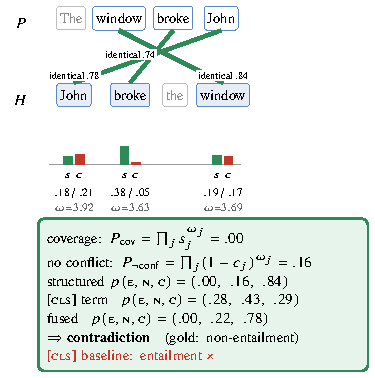
\includegraphics[width=\columnwidth]{figures/explanations/en_cover_1_compact.pdf}
  \caption{A \model{} decision on an AX-b pair that swaps the verb's arguments (RoBERTa-large, seed 1001).
  Lines: alignment (width: attention; label: relation). Bars: support $s_j$, conflict $c_j$, weight
  $\omega_j$. No word is supported in its role, so $\Pcov\approx0$ (not entailed); \cls{} predicts
  entailment.}
  \label{fig:interpretability}
\end{figure}

% Flush the floats before the conclusion (remove once the section has text).
\clearpage

\FloatBarrier
\section{Conclusion}
\label{sec:conclusion}

We presented \model{}, which decides NLI from the coverage of each hypothesis word by the premise and
from conflicts between them, using contextual token states aligned through typed lexical relations. The
structured decision is added to the logits of the standard classifier, at a cost of about 2M parameters.

Across English and Portuguese, with large encoders, 10 seeds and paired tests, \model{} matches the
\cls{} baseline in distribution and improves on it out of distribution, by up to 8.6 MCC points in English
and 2.3 in Portuguese, with lower variance across seeds. In English it also outperforms three
knowledge-graph baselines, which fall below \cls{} out of distribution.

In English, the ablation locates the effect in the coverage term and the logical aggregation; in
Portuguese, with a larger encoder, no single component is needed; the conflict term,
the lexicon and its source contribute little. The AX-b analysis shows where the rule helps, on argument
structure and logical operators, and where it fails, on restrictivity, universal quantifiers and
downward monotonicity.

Two directions follow. Extending coverage with the monotonicity of the context would address its main
failure mode, and the conflict term needs either a different training signal or removal. Cross-lingual
transfer is the weak point: the structured branch learned in English does not transfer to Portuguese,
and from Portuguese to English its gains shrink to ConjNLI.
\todo{revise when experiment 0014 finishes (Portuguese and cross-lingual baselines).}

% Required by ACL Rolling Review: unnumbered, after the conclusion and before the references;
% does not count towards the page limit.
\section*{Limitations}
\todo{Required by ARR. E.g.: two languages only; lexicon coverage differs across languages;
large Portuguese encoder trained with 8-bit optimizer states; binary metrics on the ASSIN sets.}


\bibliography{refs}

\end{document}
